\subsection{Representation}

Let us now discover two ways to represent graphs in memory,
and find out their respective advantages.

\subsubsection{Adjacency matrix}

The adjacency matrix is a two-dimensional array \texttt{a},
such that the element
\[
	\texttt{a[i][j]} =
	\begin{cases}
		1 & \text{if there is an edge from $i$ to $j$,}\\
		0 & \text{otherwise}.
	\end{cases}
\]
note that for an undirected graph, \texttt{a} is symmetric.

Let us take our first example again:

\begin{center}
	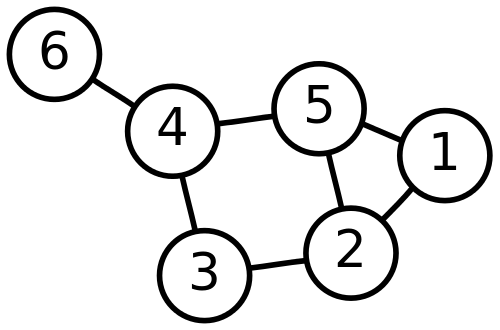
\includegraphics[width=0.3\textwidth]{img/6n-graph}
\end{center}

The corresponding adjacency matrix is:
\[
	\begin{pmatrix}
		0&1&0&0&1&0\\
		1&0&1&0&1&0\\
		0&1&0&1&0&0\\
		0&0&1&0&1&1\\
		1&1&0&1&0&0\\
		0&0&0&1&0&0\\
	\end{pmatrix}
\]

For non-simple graphs, 1 is replaced by the number of edges
joining the vertices (loops count twice).

\subsubsection{Adjacency list}

The adjacency list contains for each vertice a list
of all its neighbours.

For the same example, the adjacency list is:
\[
	\left\{
		\begin{array}{rl}
			1:&2,5\\
			2:&1,3,5\\
			3:&2,4\\
			4:&3,5,6\\
			5:&1,2,4\\
			6:&4\\
		\end{array}
	\right.
\]

The order of the neighbours does not matter.

\subsubsection{Comparison}

In terms of memory usage,
adjacency lists will generally be more compact for sparse graphs,
since it will only store data for existing edges,
while adjacency matrices will store a bit for every pair of vertices.
But for near-complete graphs, adjacency matrices will be more space-efficient.

As for time, it depends on the kind of operation you have to do.
In many cases, you have to visit all neightbours of a node,
so adjacency lists are faster,
but if you often check whether two nodes are adjacent,
the adjacency matrix is more appropriate.
